% Sections/section1.tex

\begin{frame}{Introduction to Database Security Issues (1)}
    \Large
    
    \begin{itemize}
     \vspace{-1.5 cm}
        \item \textbf{Types of Security:}
        \vspace{0.3cm}
        
        \begin{itemize}
            \large 
            \setlength{\itemsep}{0.25cm}
            
            \item \textbf{Legal and ethical issues:} \textit{e.g., GDPR, HIPAA regulations on personal data protection.}
            
            \item \textbf{Policy issues:} \textit{e.g., company rules on who can access payroll data.}
            
            \item \textbf{System-related issues:} \textit{e.g., choosing security at hardware, OS, or DBMS level.}
            
            \item \textbf{Multiple security levels:} \textit{e.g., classifying data as Public, Confidential, or Top Secret.}
        \end{itemize}
    \end{itemize}
    
\end{frame}


\begin{frame}{Introduction to Database Security Issues (2)}
    \Large
    
    \begin{itemize}
    \vspace{-1.5 cm}
        \item \textbf{Three Basic Concepts:}
        \vspace{0.3cm}
        
        \begin{itemize}
            \large
            \setlength{\itemsep}{0.4cm}
            
            \item \textbf{Authentication} \textit a mechanism that determines whether a user is who he or she claims to be.
            
            \item \textbf{Authorization} \textit the granting of a right or privilege, which enables a subject to legitimately have access to a system or a system's objects.
            
            \item \textbf{Access Control} \textit a security mechanism (of a DBMS) for restricting access to a system's objects (the database) as a whole.
        \end{itemize}
    \end{itemize}
\end{frame}

\begin{frame}{Introduction to Database Security Issue (3)}
    \Large
    
    \begin{itemize}
     \vspace{-1.5 cm}
        \item \textbf{Threats:}
        \vspace{0.3cm}
        
        \begin{itemize}
            \large
            \setlength{\itemsep}{0.4cm}
            
            \item Any situation or event, whether intentional or unintentional, that will adversely affect a system and consequently an organization.
            
            \item Threats to:
            \vspace{0.2cm}
            
            \begin{itemize}
                \normalsize
                \setlength{\itemsep}{0.2cm} 
                
                \item Computer systems
                \item Databases
            \end{itemize}
            
        \end{itemize}
    \end{itemize}
\end{frame}


% --- Slide Mới chèn thêm: Threats to Computer Systems ---
\begin{frame}[plain]
    \begin{columns}
        \begin{column}{0.4\textwidth}
            \vspace{1cm}
            \Huge \textbf{\color{green!40!black} Threats to \\[0.3cm] Computer \\[0.3cm] Systems}
        \end{column}
        
        \begin{column}{0.6\textwidth}
            \centering
            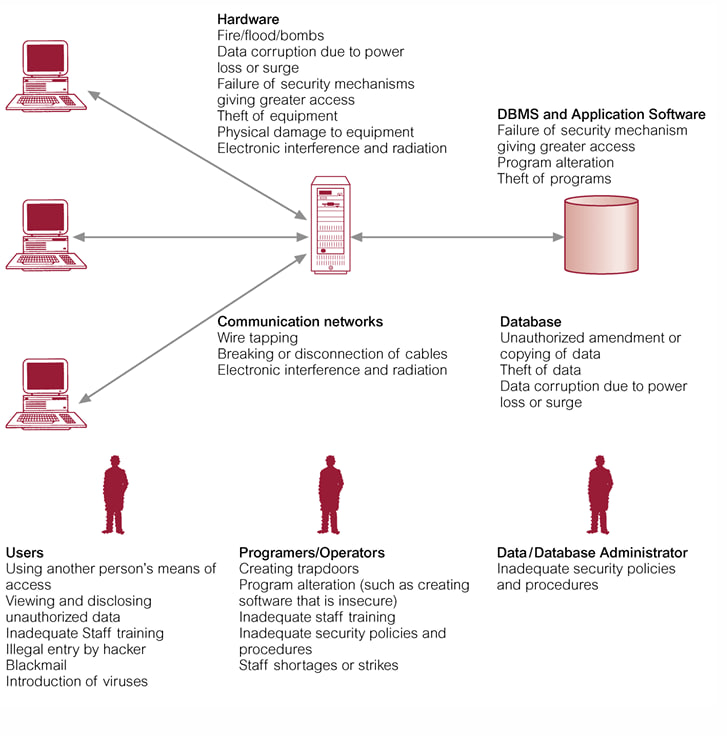
\includegraphics[width=\textwidth]{Assets/introduction3.jpg}
        \end{column}
    \end{columns}
\end{frame}


\begin{frame}{Introduction to Database Security Issues (4)}
    \Large
    
    \begin{itemize}
        
        \item \textbf{Threats to databases:}
        \vspace{0.2cm}
        \begin{itemize}
            \large 
            \setlength{\itemsep}{0.1cm}
            \item Loss of \textbf{integrity}
            \item Loss of \textbf{availability}
            \item Loss of \textbf{confidentiality}
        \end{itemize}
        
        \vspace{0.4cm}
        
        \item To protect databases against these types of threats four kinds of countermeasures can be implemented:
        \vspace{0.2cm}
        \begin{itemize}
            \large
            \setlength{\itemsep}{0.1cm}
            \item \textbf{Access control}
            \item \textbf{Inference control}
            \item \textbf{Flow control}
            \item \textbf{Encryption}
        \end{itemize}
        
    \end{itemize}
\end{frame}


\begin{frame}{Introduction to Database Security Issues (5)}
    \Large
    
    \begin{itemize}
        \vspace{-0.7cm}
        
        \item A DBMS typically includes a database security and authorization subsystem that is responsible for ensuring the security portions of a database against unauthorized access.
        
        \vspace{0.4cm}
        
        \item Two types of database security mechanisms:
        \vspace{0.2cm}
        
        \begin{itemize}
            \large
            \setlength{\itemsep}{0.3cm}
            
            \item \textbf{Discretionary} security mechanisms
            \begin{itemize}
                \normalsize
                \item \textit{Example:} The owner of a table grants \texttt{SELECT} privilege to specific users via \texttt{GRANT SELECT ON Employee TO Alice;}
            \end{itemize}
            
            \item \textbf{Mandatory} security mechanisms
            \begin{itemize}
                \normalsize
                \item \textit{Example:} Data is classified as \textit{Top Secret / Secret / Public}; a user with \textit{Secret} clearance cannot read \textit{Top Secret} data, regardless of the owner's wish.
            \end{itemize}
        \end{itemize}
        
    \end{itemize}
\end{frame}

\begin{frame}{Introduction to Database Security Issues (6)}
    \Large
    
    \begin{itemize}
        \vspace{-1.5cm}
        
        \item The security mechanism of a DBMS must include provisions for restricting access to the database as a whole
        
        \vspace{0.4cm}
        
        \begin{itemize}
            \large
            \setlength{\itemsep}{0.2cm} 
            
            \item This function is called \textbf{access control} and is handled by creating user accounts and passwords to control login process by the DBMS.
        \end{itemize}
        
    \end{itemize}
\end{frame}


\begin{frame}{Introduction to Database Security Issues (7)}
    \Large 
    
    \begin{itemize}
        \vspace{-1.5cm} 
        
        \item The security problem associated with databases is that of controlling the access to a \textbf{statistical database}, which is used to provide statistical information or summaries of values based on various criteria.
        
        \vspace{0.5cm} 
        
        \setbeamertemplate{itemize subitem}{\scriptsize$\circ$} 
        
        \begin{itemize}
            \large 
            \setlength{\itemsep}{0.2cm}
            
            \item The countermeasures to \textbf{statistical database security} problem is called \textbf{inference control measures}.
        \end{itemize}
        
    \end{itemize}
\end{frame}

% --- CẤU HÌNH SUBITEM TỪ ĐÂY TRỞ ĐI ---
\setbeamertemplate{itemize subitem}{\scriptsize$\circ$} 


% =========================================================
% === SLIDE: Statistical Database - Example & Vulnerability ===
% =========================================================
\begin{frame}{Statistical Database - Example \& Vulnerability}
    \Large
    
    \begin{itemize}
        
        \item \textbf{Example:} A university database stores individual salary records but only allows queries like \textit{AVG}, \textit{SUM}, \textit{COUNT} on groups of employees.
        
        \vspace{0.3cm}
        
        \item \textbf{Security vulnerability - Inference Attack:}
        \begin{itemize}
            \large
            \setlength{\itemsep}{0.15cm}
            
            \item Query 1: {\small\texttt{SELECT COUNT(*) FROM Emp WHERE Dept='CS' AND Gender='F'}} \\
            $\rightarrow$ Result: \textbf{1}
            
            \item Query 2: {\small\texttt{SELECT AVG(Salary) FROM Emp WHERE Dept='CS' AND Gender='F'}} \\
            $\rightarrow$ Returns the salary of that \textbf{one specific person}!
            
            \item $\Rightarrow$ Attacker infers \textbf{individual data} from aggregate queries.
        \end{itemize}
    \end{itemize}
\end{frame}

% =========================================================
% === SLIDE MỚI: Inference Control Measures ===
% =========================================================
\begin{frame}{Inference Control Measures}
    \Large
    
    \begin{itemize}
        \vspace{-0.5cm}
        \item \textbf{Common techniques to prevent inference attacks:}
        \vspace{0.2cm}
        
        \begin{itemize}
            \large
            \setlength{\itemsep}{0.2cm}
            
            \item \textbf{Query Set Size Control:} reject queries whose result set is too small (e.g., less than 5 records).
            
            \item \textbf{Query Restriction / Auditing:} log queries and block suspicious query sequences.
            
            \item \textbf{Data Perturbation:} slightly modify data values (add noise) before returning results.
            
            \item \textbf{Data Swapping:} exchange values between records while preserving statistical properties.
            
            \item \textbf{Differential Privacy:} add mathematically calibrated noise to guarantee individual privacy (modern approach used by Apple, Google).
        \end{itemize}
    \end{itemize}
\end{frame}

% =========================================================
% === SLIDE: Flow Control (có ví dụ) ===
% =========================================================
\begin{frame}{Introduction to Database Security Issues (8)}
    \Large
    
    \begin{itemize}
        \vspace{-0.5cm}
        \item Another security is that of \textbf{flow control}, which prevents information from flowing in such a way that it reaches unauthorized users.
        
        \vspace{0.4cm}
        
        \begin{itemize}
            \large
            \setlength{\itemsep}{0.2cm}
            \item \textit{Example:} A low-clearance user reads a ``Public'' report, but the report was generated from ``Top Secret'' data $\rightarrow$ information has \textbf{leaked} through an improper flow.
        \end{itemize}
        
    \end{itemize}
\end{frame}


% =========================================================
% === SLIDE: Covert Channels (có ví dụ) ===
% =========================================================
\begin{frame}{Introduction to Database Security Issues (9)}
    \Large
    
    \begin{itemize}
        \vspace{-0.5cm}
        \item Channels that are pathways for information to flow implicitly in ways that violate the security policy of an organization are called \textbf{covert channels}.
        
        \vspace{0.4cm}
        
        \begin{itemize}
            \large
            \setlength{\itemsep}{0.2cm}
            \item \textit{Example:} A high-privilege process encodes secret data by \textbf{varying CPU usage} or \textbf{locking/unlocking a shared file} in a pattern. A low-privilege process observes the pattern and decodes the secret --- \textbf{without ever directly reading it}.
        \end{itemize}
        
    \end{itemize}
\end{frame}


\begin{frame}{Introduction to Database Security Issues (10)}
    \Large
    
    \begin{itemize}
        \vspace{-1.5cm}
        
        \item A final security issue is \textbf{data encryption}, which is used to protect sensitive data (such as credit card numbers) that is being transmitted via some type communication network.
        
        \vspace{0.4cm}
        
        \item The data is \textbf{encoded} using some \textbf{encoding algorithm}.
        
        \begin{itemize}
            \large
            \setlength{\itemsep}{0.2cm}
            
            \item An unauthorized user who access encoded data will have difficulty deciphering it, but authorized users are given decoding or decrypting algorithms (or keys) to decipher data.
        \end{itemize}
        
    \end{itemize}
\end{frame}


% =========================================================
% === 4 SLIDES MỚI VỀ DATA ENCRYPTION ===
% =========================================================

% --- Slide Encryption 1: Introduction (có hình) ---
\begin{frame}{Data Encryption (1) - Introduction}
    \Large
    
    \begin{itemize}
         \vspace{-0.5cm}
        \item \textbf{Encryption} protects sensitive data by encoding it so that only authorized users with the correct key can decipher it.
    \end{itemize}
    
    \vspace{0.3cm}
    \centering
    % Bạn nhớ sửa tên file 'encryption3.jpg' thành đúng tên ảnh của bạn trong thư mục Assets nhé!
    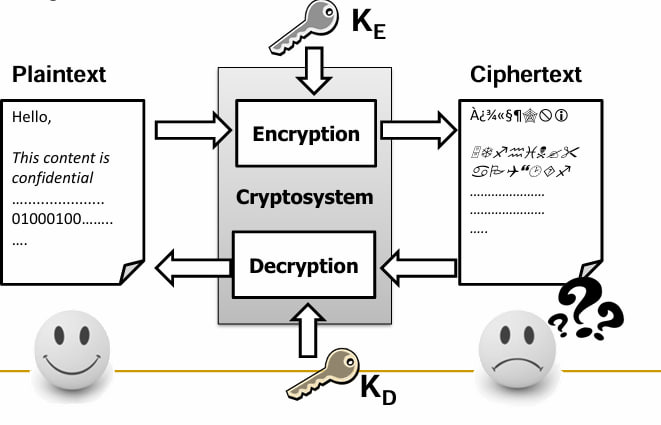
\includegraphics[width=0.6\textwidth]{Assets/encryption3.jpg}
\end{frame}


% --- Slide Encryption 2: Mục tiêu bảo vệ ---
\begin{frame}{Data Encryption (2) - Protection Goals}
    \Large
    
    \begin{itemize}
        \vspace{-1.2cm}
        
        \item \textbf{Two main protection goals:}
        \begin{itemize}
            \large
            \setlength{\itemsep}{0.3cm}
            
            \item \textbf{Data at-rest:} protecting data stored on disks, backups, or database files.
            \begin{itemize}
                \normalsize
                \item \textit{Example:} Encrypting the entire database file using \textbf{Transparent Data Encryption (TDE)} in SQL Server / Oracle.
            \end{itemize}
            
            \item \textbf{Data in-transit:} protecting data while being transmitted over networks.
            \begin{itemize}
                \normalsize
                \item \textit{Example:} Using \textbf{TLS/SSL} when a client connects to a database server.
            \end{itemize}
        \end{itemize}
    \end{itemize}
\end{frame}


% --- Slide Encryption 3: Các kỹ thuật điển hình ---
\begin{frame}{Data Encryption (3) - Classic Techniques}
    \Large
    
    \begin{itemize}
        
        \item \textbf{Symmetric Encryption:} same key for encryption and decryption.
        \begin{itemize}
            \large
            \setlength{\itemsep}{0.1cm}
            \item \textbf{AES} (Advanced Encryption Standard) - industry standard, 128/192/256-bit.
            \item \textbf{DES / 3DES} - older, largely replaced by AES.
        \end{itemize}
        
        \vspace{0.2cm}
        
        \item \textbf{Asymmetric Encryption:} uses a public key + private key pair.
        \begin{itemize}
            \large
            \setlength{\itemsep}{0.1cm}
            \item \textbf{RSA} - widely used for key exchange and digital signatures.
            \item \textbf{ECC} (Elliptic Curve Cryptography) - stronger security with smaller keys.
        \end{itemize}
        
        \vspace{0.2cm}
        
        \item \textbf{Hashing:} one-way function for password storage and integrity check.
        \begin{itemize}
            \large
            \item \textbf{SHA-256}, \textbf{bcrypt}, \textbf{Argon2}.
        \end{itemize}
    \end{itemize}
\end{frame}

% --- Slide Encryption 4: Xu hướng hiện đại ---
\begin{frame}{Data Encryption (4) - Modern Trends}
    \Large
    
    \begin{itemize}
        
        \item \textbf{Homomorphic Encryption:}
        \begin{itemize}
            \large
            \item Allows computation \textbf{directly on encrypted data} without decrypting it.
            \item \textit{Example:} A cloud server can compute \texttt{SUM(salary)} on encrypted data and return an encrypted result --- the server never sees the plaintext.
        \end{itemize}
        
        \vspace{0.2cm}
        
        \item \textbf{End-to-End Encryption (E2EE):}
        \begin{itemize}
            \large
            \item Data is encrypted on the sender's device and only decrypted on the receiver's device (e.g., Signal, WhatsApp).
        \end{itemize}
        
        \vspace{0.2cm}
        
        \item \textbf{Post-Quantum Cryptography:}
        \begin{itemize}
            \large
            \item New algorithms (e.g., \textbf{CRYSTALS-Kyber}, \textbf{Dilithium}) designed to resist attacks from future \textbf{quantum computers}.
            \item Standardized by NIST in 2024.
        \end{itemize}
    \end{itemize}
\end{frame}


\begin{frame}{Database Security and the DBA (1)}
    \Large
    
    \begin{itemize}
        \vspace{-1.5cm}
        
        \item The database administrator (\textbf{DBA}) is the central authority for managing a database system.
        
        \begin{itemize}
            \large
            \setlength{\itemsep}{0.2cm}
            
            \item The DBA's responsibilities include:
            
            \begin{itemize}
                \normalsize
                \setlength{\itemsep}{0.1cm}
                
                \item granting privileges to users who need to use the system.
                \item classifying users and data in accordance with the policy of the organization.
            \end{itemize}
        \end{itemize}
        
        \vspace{0.4cm}
        
        \item The DBA is responsible for the overall security of the database system.
        
    \end{itemize}
\end{frame}


\begin{frame}{Database Security and the DBA (2)}
    \Large
    
    \begin{itemize}
        \vspace{-1.5cm}
        
        \item The DBA has a DBA account in the DBMS:
        
        \begin{itemize}
            \large
            \setlength{\itemsep}{0.2cm}
            
            \item Sometimes these are called a system or superuser account.
            
            \item These accounts provide powerful capabilities such as:
            
            \begin{itemize}
                \normalsize
                \setlength{\itemsep}{0.1cm}
                
                \item 1. Account creation
                \item 2. Privilege granting
                \item 3. Privilege revocation
                \item 4. Security level assignment
            \end{itemize}
            
            \item Action 1 is access control, whereas 2 and 3 are discretionary and 4 is used to control mandatory authorization.
            
        \end{itemize}
        
    \end{itemize}
\end{frame}


\begin{frame}{Access Protection, User Accounts, and Database Audits (1)}
    \Large
    
    \begin{itemize}
        \vspace{-1.5cm}
        
        \item Whenever a person or group of persons need to access a database system, the individual or group must first apply for a user account.
        
        \begin{itemize}
            \large
            \setlength{\itemsep}{0.2cm}
            
            \item The DBA will then create a new \textbf{account id} and \textbf{password} for the user if he/she deems there is a legitimate need to access the database.
        \end{itemize}
        
        \vspace{0.4cm}
        
        \item The user must log in to the DBMS by entering account id and password whenever database access is needed.
        
    \end{itemize}
\end{frame}


\begin{frame}{Access Protection, User Accounts, and Database Audits (2)}
    \Large
    
    \begin{itemize}
        \vspace{-1.5cm}
        
        \item The database system must also keep \textbf{track of all operations} on the database that are applied by a certain user throughout \textbf{each login session}.
        
        \vspace{0.4cm}
        
        \begin{itemize}
            \large
            \setlength{\itemsep}{0.2cm}
            
            \item To keep a record of all updates applied to the database and of the particular user who applied each update, we can modify \textbf{system log}, which includes an entry for each operation applied to the database that may be required for recovery from a transaction failure or system crash.
        \end{itemize}
        
    \end{itemize}
\end{frame}


\begin{frame}{Access Protection, User Accounts, and Database Audits (3)}
    \Large
    
    \begin{itemize}
        \vspace{-1.5cm}
        
        \item If any tampering with the database is suspected, a \textbf{database audit} is performed.
        
        \begin{itemize}
            \large
            \setlength{\itemsep}{0.2cm}
            
            \item A database audit consists of reviewing the log to examine all accesses and operations applied to the database during a certain time period.
        \end{itemize}
        
        \vspace{0.4cm}
        
        \item A database log that is used mainly for security purposes is sometimes called an \textbf{audit trail}.
        
    \end{itemize}
\end{frame}
